% Hardware IP technical presentation manuscript.
% Compile with XeLaTeX. This file is independent from main.tex.

\documentclass[fontset=fandol,ugly,language=chinese]{pkuthss}

\usepackage{booktabs,longtable,makecell,multirow}
\usepackage{amsmath}
\usepackage{enumitem}
\usepackage{tikz}
\usetikzlibrary{arrows.meta,positioning,fit,calc,backgrounds}
\usepackage{hyperref}

\setlist[itemize]{leftmargin=2em,itemsep=0.25em}
\setlist[enumerate]{leftmargin=2.3em,itemsep=0.25em}

\newcommand{\module}[1]{\texttt{#1}}
\newcommand{\signal}[1]{\texttt{#1}}
\newcommand{\KTILE}{K_{\mathrm{TILE}}}
\newcommand{\COUTTILE}{COUT_{\mathrm{TILE}}}
\newcommand{\KTOTAL}{K_{\mathrm{total}}}
\newcommand{\COUT}{C_{\mathrm{out}}}
\newcommand{\CIN}{C_{\mathrm{in}}}

\pkuthssinfo{
    ctitle = {卷积神经网络 FPGA 加速器硬件 IP 技术报告},
    etitle = {Technical Report for CNN FPGA Accelerator Hardware IP Design},
}

\begin{document}
\frontmatter
\pagestyle{plain}

\begin{center}
    {\zihao{2}\heiti 卷积神经网络 FPGA 加速器硬件 IP 技术报告}

    \vspace{1em}
    {\zihao{4}基于权重驻留脉动阵列的轻量级 CNN INT8 卷积加速器}
\end{center}

\vspace{1em}

本文档面向硬件 IP 设计部分的 PowerPoint 汇报准备，但不采用简单提纲形式，而是按照技术报告体例展开。每一章均围绕一组可转化为 PPT 的核心页面组织：先给出本章适合放入 PPT 的展示重点，再展开必要的理论公式、结构框图、模块职责、数据流语义和实现约束。内容限定在 PL 侧硬件 IP 逻辑，包括卷积映射、脉动阵列、输入窗口生成、三级分块调度、PSUM 反馈、后处理流水线、AXI 边界、验证和资源评估；PS 端软件驱动和完整系统集成只作为接口契约背景，不作为主体展开。

\tableofcontents

\mainmatter

\chapter{背景、目标与汇报主线}

\section{PPT 展示重点}

\begin{itemize}
    \item 边缘侧目标检测需要在有限功耗和有限 FPGA 资源下完成 CNN 推理。
    \item 卷积层是 YOLOv3-tiny 等轻量化网络中的主要计算瓶颈。
    \item 本工作设计的是一个可综合、可验证、带标准接口边界的 INT8 卷积加速硬件 IP。
    \item 核心路线：卷积到分块 GEMM 映射 + weight-stationary 脉动阵列 + K/Cout/Spatial 三级分块。
    \item 最终资源点：XCK26 上采用 18$\times$16 阵列，$\KTILE=18$，$\COUTTILE=32$。
\end{itemize}

\section{问题背景}

卷积神经网络在目标检测、图像分类和语义分割中已经成为主流计算模型，但其推理过程包含大量乘加运算。以 YOLOv3-tiny 为代表的轻量化网络虽然已经降低了层数和参数量，但卷积层仍然承担主要计算量。对于边缘设备，推理系统同时受到以下约束：

\begin{itemize}
    \item \textbf{吞吐约束}：输入图像需要在较短延迟内完成前向推理，目标检测类任务通常要求稳定帧率。
    \item \textbf{功耗约束}：嵌入式平台不适合使用高功耗 GPU，CPU 又难以提供足够的并行乘加吞吐。
    \item \textbf{片上资源约束}：目标 FPGA 器件的 LUT、DSP、BRAM 和片上互连资源有限，不能简单堆叠大型阵列。
    \item \textbf{数据搬运约束}：CNN 推理不仅受算力限制，也受外部存储带宽和片上缓存复用效率影响。
\end{itemize}

因此，硬件 IP 的设计重点不是单纯实现一个乘法阵列，而是建立一条能够持续供数、可分块执行、可反馈累加、可后处理写回的卷积层数据流。

\section{设计目标}

本设计面向 Xilinx Zynq UltraScale+ XCK26 器件，目标是实现一款可作为后续系统集成基础的卷积加速硬件 IP。设计目标可概括为：

\begin{enumerate}
    \item \textbf{计算核心可扩展}：采用参数化二维脉动阵列，能够在不同 ROWS/COLS 配置下进行资源和性能折中。
    \item \textbf{卷积语义闭环}：支持 3$\times$3 卷积展开、padding、stride、bias 注入、多 pass PSUM 累加和 INT8 输出。
    \item \textbf{分块覆盖大层}：通过 K 维度、输出通道维度和空间维度三层分块，在有限阵列规模下覆盖大通道、大尺寸特征图。
    \item \textbf{接口边界清晰}：控制面采用 AXI-Lite，数据面采用 AXI-Stream 风格输入输出边界，便于连接 DMA。
    \item \textbf{验证证据完整}：从 PE、窗口提取、调度器、后处理到全链路 AXI 边界均建立自动化 testbench。
\end{enumerate}

\section{汇报主线}

建议 PPT 按以下顺序展开。这个顺序不是按 RTL 文件层次机械排列，而是按听众理解硬件 IP 的路径组织：

\begin{enumerate}
    \item \textbf{问题与目标}：为什么需要这个 IP，它解决卷积推理中的哪一类瓶颈。
    \item \textbf{数学映射}：卷积如何映射成分块 GEMM，为什么需要 K/Cout/Spatial 三维分块。
    \item \textbf{总体架构}：从 IFM 行输入到 OFM 写回的完整硬件数据流。
    \item \textbf{计算核心}：PE、双 INT8 乘法、weight-stationary 阵列和偏斜注入。
    \item \textbf{输入前端}：行缓存、窗口提取、padding/stride 和 IFM FIFO。
    \item \textbf{调度与反馈}：layer scheduler、PSUM drain、feedback buffer 和多 pass 语义。
    \item \textbf{后处理与接口}：requant、activation、HWC writeback、AXI-Lite/AXI-Stream。
    \item \textbf{验证和资源}：仿真覆盖、资源折中、最终 XCK26 结果。
\end{enumerate}

\chapter{卷积计算模型与分块 GEMM 映射}

\section{PPT 展示重点}

\begin{itemize}
    \item 标准卷积是六重循环，本 IP 将其映射为输出像素维度 $P$ 与输出通道维度 $\COUT$ 上的矩阵乘。
    \item 展开维度 $\KTOTAL=\CIN \times K_h \times K_w$ 是阵列行方向处理对象。
    \item 阵列物理规模有限，因此必须进行 K 分块、Cout 分块和 Spatial 分块。
    \item 分块设计决定了硬件资源、片上缓冲需求和外部数据服务协议。
\end{itemize}

\section{标准卷积公式}

设输入特征图为 $I[c_{in},y,x]$，权重为 $W[c_{out},c_{in},k_y,k_x]$，偏置为 $B[c_{out}]$。对步长 $S$、填充 $P_d$ 的二维卷积，有：

\begin{equation}
\begin{aligned}
O[c_{out},oy,ox] =
B[c_{out}] +
\sum_{c_{in}=0}^{\CIN-1}
\sum_{k_y=0}^{K_h-1}
\sum_{k_x=0}^{K_w-1} & I[c_{in}, oyS+k_y-P_d, oxS+k_x-P_d]\\
& \cdot W[c_{out}, c_{in}, k_y, k_x].
\end{aligned}
\label{eq:conv_basic}
\end{equation}

其中越界位置按 padding 语义视为 0。本文硬件前端主要面向 $K_h=K_w=3$ 的卷积窗口，因此窗口提取器围绕 3 行、3 列并行读取和 lane 展开设计。

\section{展开到 GEMM}

定义输出像素一维索引：

\begin{equation}
p = oy \cdot W_{out} + ox,
\label{eq:p_index}
\end{equation}

定义卷积展开维度：

\begin{equation}
k = c_{in} \cdot K_h K_w + k_y \cdot K_w + k_x,\qquad
\KTOTAL = \CIN \cdot K_h \cdot K_w.
\label{eq:k_index}
\end{equation}

则卷积可写为：

\begin{equation}
OFM[p,c] = Bias[c] + \sum_{k=0}^{\KTOTAL-1} IFM[p,k] \cdot W[k,c].
\label{eq:gemm_basic}
\end{equation}

这一形式非常适合脉动阵列：阵列行方向对应 $k$ 维度，列方向对应输出通道维度。一个输出像素 $p$ 的 IFM 展开向量从阵列左侧注入，一个输出通道块的权重驻留在 PE 内部，最终每列得到对应输出通道的 PSUM。

\section{为什么必须分块}

完整 YOLO 风格卷积层可能具有较大的通道数。若 $\CIN=512$、$K_h=K_w=3$，则：

\begin{equation}
\KTOTAL = 512 \times 3 \times 3 = 4608.
\end{equation}

这远大于当前物理阵列行数 $\KTILE=18$。同理，若 $\COUT=1024$，也远大于当前 $\COUTTILE=32$。因此，完整 GEMM 需要被切分为多个子问题：

\begin{equation}
OFM[p,c] =
Bias[c] +
\sum_{t=0}^{N_K-1}
\sum_{r=0}^{\KTILE-1}
IFM[p,t\KTILE+r] \cdot W[t\KTILE+r,c],
\label{eq:k_tiled}
\end{equation}

其中 $N_K=\lceil \KTOTAL/\KTILE \rceil$。当最后一个 K tile 不满时，越界 lane 输入为 0 或通过有效范围屏蔽，不改变最终数学语义。

\section{三级分块关系}

本设计采用的分块层次如下：

\begin{table}[htbp]
\centering
\caption{卷积层三级分块语义}
\label{tab:tiling_summary}
\begin{tabular}{lll}
\toprule
\textbf{分块维度} & \textbf{硬件参数} & \textbf{作用} \\
\midrule
K 维度 & $\KTILE=ROWS$ & 限制单 pass 覆盖的展开输入 lane 数 \\
Cout 维度 & $\COUTTILE=COLS\times2$ & 限制单 block 覆盖的输出通道数 \\
Spatial 维度 & \signal{tile\_ofm\_h}, \signal{num\_pixels} & 限制单次启动覆盖的输出像素范围 \\
\bottomrule
\end{tabular}
\end{table}

三者的调度顺序可概括为：

\begin{equation}
\text{for each spatial tile}
\rightarrow
\text{for each Cout block}
\rightarrow
\text{for each K pass}
\rightarrow
\text{compute and drain}.
\end{equation}

K 分块解决阵列行数不足问题，Cout 分块解决阵列列数不足问题，Spatial 分块解决片上 PSUM/OFM 缓冲容量不足问题。三者共同决定硬件 IP 对大规模卷积层的覆盖能力。

\begin{figure}[htbp]
\centering
\begin{tikzpicture}[
    >=Latex,
    every node/.style={font=\small},
    tile/.style={draw, fill=black!7, minimum width=2.0cm, minimum height=1.0cm, align=center},
    dim/.style={<->, thick},
    dline/.style={dashed, gray}
]
    \draw[thick] (0,0) rectangle (8,4.2);
    \node at (4,4.55) {权重矩阵 $W[\KTOTAL,\COUT]$};
    \draw[dline] (0,2.8) -- (8,2.8);
    \draw[dline] (0,1.4) -- (8,1.4);
    \draw[dline] (2.4,0) -- (2.4,4.2);
    \draw[dline] (4.8,0) -- (4.8,4.2);
    \node[tile] at (1.2,3.5) {一个\\计算 tile};
    \node at (8.7,3.5) {K pass 0};
    \node at (8.7,2.1) {K pass 1};
    \node at (8.7,0.7) {$\cdots$};
    \node at (1.2,4.85) {Cout block 0};
    \node at (3.6,4.85) {Cout block 1};
    \node at (6.4,4.85) {$\cdots$};
    \draw[dim] (-0.45,0) -- (-0.45,4.2);
    \node[rotate=90] at (-0.85,2.1) {$\KTOTAL$};
    \draw[dim] (0,-0.45) -- (8,-0.45);
    \node at (4,-0.85) {$\COUT$};
    \draw[dim] (0,4.32) -- (2.4,4.32);
    \node[above] at (1.2,4.32) {$\COUTTILE$};
    \draw[dim] (-0.2,2.8) -- (-0.2,4.2);
    \node[left] at (-0.2,3.5) {$\KTILE$};

    \begin{scope}[xshift=10.3cm,yshift=0.15cm]
        \draw[thick] (0,0) rectangle (1.1,3.9);
        \draw[dline] (0,2.6) -- (1.1,2.6);
        \draw[dline] (0,1.3) -- (1.1,1.3);
        \node at (0.55,3.25) {Tile 0};
        \node at (0.55,1.95) {Tile 1};
        \node at (0.55,0.65) {$\cdots$};
        \node[align=center,right=0.4cm] at (1.1,2.0) {Spatial\\tiles};
    \end{scope}
\end{tikzpicture}
\caption{K/Cout/Spatial 三级分块示意}
\label{fig:tiling_report}
\end{figure}

\chapter{硬件 IP 总体架构}

\section{PPT 展示重点}

\begin{itemize}
    \item IP 由前端窗口流、脉动阵列计算核心、PSUM 反馈与后处理链路组成。
    \item 控制面负责寄存器配置、start/done 和调度状态。
    \item 数据面包含 bias、weight、IFM line 和 OFM 四类数据流。
    \item 每个模块边界尽量采用 valid/ready 或 request/done 语义，便于逐步 AXI 化。
\end{itemize}

\section{总体数据流}

顶层硬件 IP 的数据流如图~\ref{fig:overall_arch_report} 所示。它不是一个单周期算子，而是一个围绕卷积层执行过程组织的流式系统：

\begin{enumerate}
    \item 外部通过 IFM line stream 按行填充 line buffer。
    \item window extractor 根据输出坐标和 K pass 基址生成并行 IFM lane。
    \item IFM FIFO 对输入 lane 进行缓冲和偏斜对齐。
    \item weight tile loader 将当前 tile 的权重写入 PE 权重寄存器。
    \item systolic array 产生当前 K pass 的 PSUM。
    \item PSUM drain 根据 pass 类型将结果送入 feedback buffer 或最终后处理链。
    \item requant、activation、writeback 产生 INT8 OFM 字节流。
\end{enumerate}

\begin{figure}[htbp]
\centering
\resizebox{\textwidth}{!}{
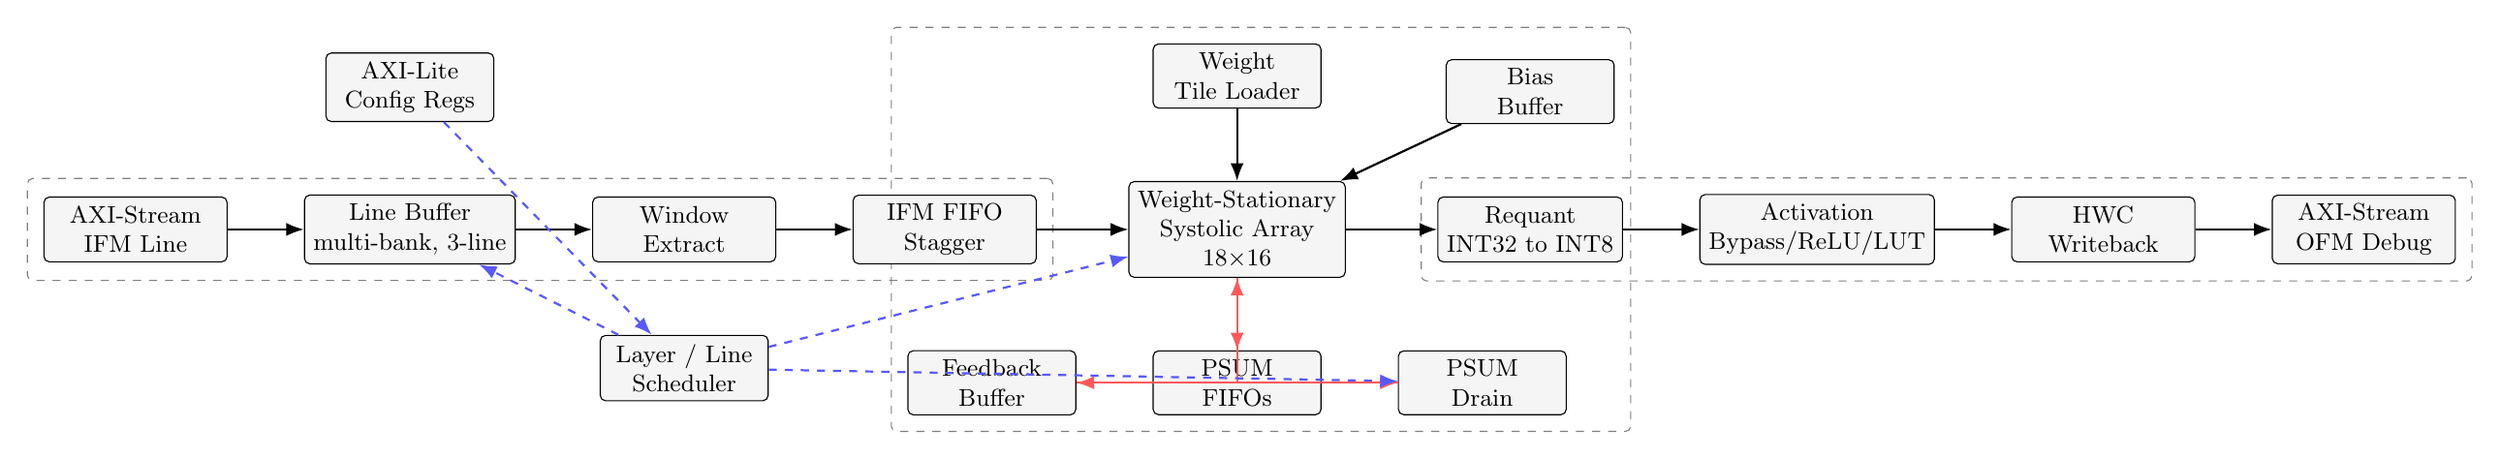
\begin{tikzpicture}[
    >=Latex,
    node distance=8mm and 10mm,
    block/.style={draw, rounded corners=2pt, align=center, minimum width=2.4cm, minimum height=0.85cm, fill=black!4, font=\small},
    small/.style={draw, rounded corners=2pt, align=center, minimum width=2.2cm, minimum height=0.75cm, fill=black!4, font=\small},
    arr/.style={->, thick},
    ctrl/.style={->, thick, dashed, blue!65},
    psum/.style={->, thick, red!65},
    group/.style={draw, dashed, rounded corners=2pt, inner sep=6pt, gray}
]
    \node[block] (axis_ifm) {AXI-Stream\\IFM Line};
    \node[block, right=of axis_ifm] (linebuf) {Line Buffer\\multi-bank, 3-line};
    \node[block, right=of linebuf] (window) {Window\\Extract};
    \node[block, right=of window] (ifmfifo) {IFM FIFO\\Stagger};
    \node[block, right=1.2cm of ifmfifo, minimum width=2.7cm, minimum height=1.15cm] (array) {Weight-Stationary\\Systolic Array\\18$\times$16};
    \node[block, right=1.2cm of array] (requant) {Requant\\INT32 to INT8};
    \node[block, right=of requant] (act) {Activation\\Bypass/ReLU/LUT};
    \node[block, right=of act] (wb) {HWC\\Writeback};
    \node[block, right=of wb] (ofm) {AXI-Stream\\OFM Debug};

    \node[small, above=0.95cm of array] (wgt) {Weight\\Tile Loader};
    \node[small, above=0.95cm of requant] (bias) {Bias\\Buffer};
    \node[small, below=0.95cm of array] (psumfifo) {PSUM\\FIFOs};
    \node[small, right=of psumfifo] (drain) {PSUM\\Drain};
    \node[small, left=of psumfifo] (fb) {Feedback\\Buffer};
    \node[small, below=0.95cm of window] (sched) {Layer / Line\\Scheduler};
    \node[small, above=0.95cm of linebuf] (cfg) {AXI-Lite\\Config Regs};

    \draw[arr] (axis_ifm) -- (linebuf);
    \draw[arr] (linebuf) -- (window);
    \draw[arr] (window) -- (ifmfifo);
    \draw[arr] (ifmfifo) -- (array);
    \draw[arr] (array) -- (requant);
    \draw[arr] (requant) -- (act);
    \draw[arr] (act) -- (wb);
    \draw[arr] (wb) -- (ofm);

    \draw[arr] (wgt) -- (array);
    \draw[arr] (bias) -- (array);
    \draw[psum] (array) -- (psumfifo);
    \draw[psum] (psumfifo) -- (drain);
    \draw[psum] (drain) -- (fb);
    \draw[psum] (fb) -| (array);
    \draw[ctrl] (cfg) -- (sched);
    \draw[ctrl] (sched) -- (linebuf);
    \draw[ctrl] (sched) -- (array);
    \draw[ctrl] (sched) -- (drain);

    \begin{scope}[on background layer]
        \node[group, fit=(axis_ifm)(linebuf)(window)(ifmfifo)] {};
        \node[group, fit=(array)(wgt)(bias)(psumfifo)(drain)(fb)] {};
        \node[group, fit=(requant)(act)(wb)(ofm)] {};
    \end{scope}
\end{tikzpicture}}
\caption{硬件 IP 总体架构与主要数据通路}
\label{fig:overall_arch_report}
\end{figure}

\section{模块职责划分}

\begin{longtable}{p{0.34\textwidth}p{0.56\textwidth}}
\caption{主要 RTL 模块职责}\\
\toprule
\textbf{模块} & \textbf{职责} \\
\midrule
\endfirsthead
\toprule
\textbf{模块} & \textbf{职责} \\
\midrule
\endhead
\module{layer\_config\_regs} & 保存卷积层尺寸、stride/pad、K/Cout 总量、spatial tile 参数和启动/完成状态。\\
\module{layer\_scheduler\_stream} & 按 Cout block 和 K pass 组织 bias load、weight load、feeder、compute、drain 的执行顺序。\\
\module{line\_buffer\_5bank} & 保存窗口提取所需输入行，提供每行三个水平读端口。\\
\module{window\_extract} & 根据 $(oy,ox)$、stride、pad、\signal{pass\_base\_k} 展开 IFM lane。\\
\module{systolic\_pe} & 单个 PE，包含双权重寄存器、IFM 传播、PSUM 累加和 valid 对齐。\\
\module{systolic\_array\_32x32} & 参数化二维 PE 网格，当前用于 18$\times$16、16$\times$16、32$\times$16 等配置。\\
\module{psum\_drain\_writer} & 从阵列底部 PSUM FIFO 读取 packet，区分 partial PSUM 和 final PSUM。\\
\module{ofm\_requant\_writer} & 对 final PSUM packet 并行执行重量化。\\
\module{ofm\_activation} & 支持 bypass、ReLU 和 LUT 型 Leaky 激活。\\
\module{ofm\_writeback} & 将 OFM packet 展开为 HWC 布局下的字节写地址和数据。\\
\bottomrule
\end{longtable}

\section{控制面与数据面的分离}

该 IP 的一个重要设计原则是控制面和数据面分离。AXI-Lite 或本地配置总线只负责写寄存器和读状态，数据搬运则通过请求信号与 AXI-Stream 边界完成。这样做有两个好处：

\begin{itemize}
    \item 计算核心不依赖某一种具体 DMA 控制器实现，可以先通过 testbench 直接服务请求，再逐步替换为 AXI-Stream wrapper。
    \item 调度语义清晰：硬件只发出 \signal{bias\_load\_req}、\signal{weight\_load\_req}、\signal{feeder\_fill\_req} 等请求，外部服务端按协议提供数据。
\end{itemize}

在 PPT 中建议用一页讲清楚“核心计算链路保持稳定，外部接口逐层封装”的设计路线。RTL 的封装层次可概括为：基础寄存器核向外逐步增加 AXI-Lite、ready-valid stream 和完整 AXI-Stream 边界，最终形成正式 AXI 边界顶层。

\chapter{Weight-Stationary 脉动阵列计算核心}

\section{PPT 展示重点}

\begin{itemize}
    \item 选择 weight-stationary 数据流，使权重在 PE 内驻留，IFM 横向流动，PSUM 纵向累加。
    \item 每个 PE 驻留两个 INT8 权重，对应同一列的两个输出通道。
    \item 阵列规模为 ROWS$\times$COLS，输出通道 tile 为 $COLS\times2$。
    \item 18$\times$16 配置下峰值吞吐为 57.6 GOPS@100 MHz。
    \item IFM 和 PSUM 的 valid 信号随流水线传播，保证有效数据才参与累加。
\end{itemize}

\section{PE 计算语义}

对于第 $r$ 行、第 $c$ 列 PE，内部驻留两个权重 $w_{r,2c}$ 和 $w_{r,2c+1}$。当输入 lane $x_r$ 与来自上方的部分和 $s_{2c}$、$s_{2c+1}$ 到达时，PE 执行：

\begin{align}
s'_{2c} &= s_{2c} + x_r \cdot w_{r,2c},\\
s'_{2c+1} &= s_{2c+1} + x_r \cdot w_{r,2c+1}.
\end{align}

其中 $x_r$ 为当前输出像素在 K tile 内第 $r$ 个展开输入值。对一列 PE 来说，PSUM 从第 0 行依次经过 ROWS 个 PE，最终在底部得到该 K tile 对两个输出通道的累加贡献。

\section{PE 结构框图}

\begin{figure}[htbp]
\centering
\begin{tikzpicture}[
    >=Latex,
    node distance=8mm,
    box/.style={draw, rounded corners=2pt, align=center, minimum width=2.6cm, minimum height=0.8cm, fill=black!5},
    reg/.style={draw, rounded corners=2pt, align=center, minimum width=1.5cm, minimum height=0.65cm, fill=white},
    arr/.style={->, thick}
]
    \node[box, minimum width=3.5cm, minimum height=2.0cm] (mul) {Dual INT8\\Multiply\\$x\cdot w_0$, $x\cdot w_1$};
    \node[reg, above left=0.5cm and 0.3cm of mul] (w0) {$w_0$};
    \node[reg, below left=0.5cm and 0.3cm of mul] (w1) {$w_1$};
    \node[box, right=1.2cm of mul] (acc) {PSUM\\Add};
    \node[left=1.0cm of mul] (ifmin) {IFM in};
    \node[right=1.0cm of acc] (ifmout) {IFM out};
    \node[above=1.0cm of acc] (psumtop) {PSUM in};
    \node[below=1.0cm of acc] (psumbot) {PSUM out};

    \draw[arr] (ifmin) -- (mul);
    \draw[arr] (mul) -- node[above]{product} (acc);
    \draw[arr] (mul.east) -- ++(0.35,0) |- (ifmout);
    \draw[arr] (w0) -- (mul);
    \draw[arr] (w1) -- (mul);
    \draw[arr] (psumtop) -- (acc);
    \draw[arr] (acc) -- (psumbot);
    \node[align=left, font=\small, below=1.0cm of mul] {valid\_h 随 IFM 横向延迟\\valid\_v 随 PSUM 纵向延迟};
\end{tikzpicture}
\caption{PE 内部数据通路抽象}
\label{fig:pe_report}
\end{figure}

\section{阵列级数据流}

阵列级数据流可以理解为二维时空调度：

\begin{itemize}
    \item \textbf{权重加载}：权重 tile 按 $r \times \COUTTILE + lane$ 的顺序写入 tile buffer，再按列加载到 PE 权重寄存器。
    \item \textbf{IFM 注入}：第 $r$ 行 IFM FIFO 的读使能相对第 0 行延迟，使不同 lane 在阵列内部与对应 PSUM 对齐。
    \item \textbf{PSUM 注入}：第一 K pass 顶部注入 bias；后续 K pass 顶部注入上一 pass 的 partial sum。
    \item \textbf{结果排出}：阵列底部每列输出两个 PSUM lane，经 PSUM FIFO 缓冲后交给 drain writer。
\end{itemize}

\begin{figure}[htbp]
\centering
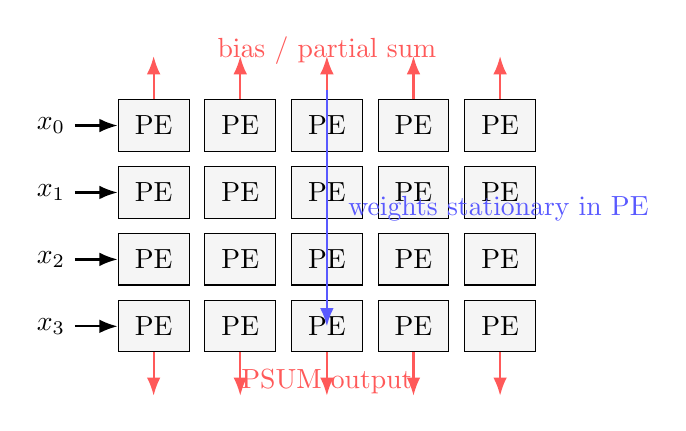
\begin{tikzpicture}[
    >=Latex,
    pe/.style={draw, minimum width=0.9cm, minimum height=0.65cm, fill=black!4},
    arr/.style={->, thick},
    warr/.style={->, thick, blue!65},
    parr/.style={->, thick, red!65}
]
    \foreach \r in {0,...,3} {
        \foreach \c in {0,...,4} {
            \node[pe] (p\r\c) at (\c*1.1,-\r*0.85) {PE};
        }
    }
    \foreach \r in {0,...,3} {
        \draw[arr] (-1.0,-\r*0.85) -- (p\r0.west);
        \node[left] at (-1.0,-\r*0.85) {$x_{\r}$};
    }
    \foreach \c in {0,...,4} {
        \draw[parr] (p0\c.north) -- ++(0,0.55);
        \draw[parr] (p3\c.south) -- ++(0,-0.55);
    }
    \node[red!65] at (2.2,0.95) {bias / partial sum};
    \node[red!65] at (2.2,-3.25) {PSUM output};
    \draw[warr] (2.2,0.45) -- (2.2,-2.55);
    \node[blue!65,right] at (2.35,-1.05) {weights stationary in PE};
\end{tikzpicture}
\caption{Weight-stationary 阵列中 IFM、权重和 PSUM 的方向}
\label{fig:array_dataflow_report}
\end{figure}

\section{吞吐与资源估算}

在 ROWS$\times$COLS 阵列中，每个 PE 每周期产生两路 INT8 乘法贡献，因此理论乘加吞吐为：

\begin{equation}
T_{\mathrm{peak}} = ROWS \times COLS \times 2 \times f_{\mathrm{clk}}.
\end{equation}

最终 18$\times$16 配置在 100 MHz 时：

\begin{equation}
T_{\mathrm{peak}} = 18 \times 16 \times 2 \times 100\mathrm{MHz}
=57.6\ \mathrm{GOPS}.
\end{equation}

该峰值只反映阵列满流水时的理论能力，实际有效吞吐还受 K pass 数、weight reload、line fill、pipeline fill/drain 和输出背压影响。PPT 中建议把峰值吞吐和有效吞吐分开说明，避免把理论上限误写成端到端性能。

\chapter{IFM 行缓存、窗口提取与输入对齐}

\section{PPT 展示重点}

\begin{itemize}
    \item 输入前端不显式生成完整 im2col 矩阵，而是按输出像素流式生成 IFM lane。
    \item 行缓存保存 3$\times$3 窗口需要的输入行，支持 padding 和 stride。
    \item 窗口提取按 $\KTILE$ 个 lane 输出给阵列行方向。
    \item IFM FIFO 同时承担缓冲和阵列偏斜注入职责。
\end{itemize}

\section{行缓存结构}

3$\times$3 卷积窗口最多同时依赖 3 行输入特征图。行缓存采用三物理行循环替换结构，每次外部填充一整行 IFM 后，通过 \signal{dma\_line\_advance} 提交该行。每个物理行提供三个读端口，分别读取当前窗口的 $x$、$x+1$、$x+2$ 三个水平位置。

bank 维度用于在通道方向拆分 IFM 数据。窗口提取时，根据 lane 对应的输入通道 $c_{in}$ 选择 bank：

\begin{equation}
bank = c_{in} \bmod N_{\mathrm{bank}}.
\end{equation}

最终资源评估中将 bank 数缩减到 2，以降低片上资源开销。若未来面向更高并行通道或更宽输入流，可重新增大 bank 数。

\section{窗口坐标生成}

对于输出坐标 $(oy,ox)$，3$\times$3 窗口中位置 $(k_y,k_x)$ 对应的输入坐标为：

\begin{align}
f_y &= oy \cdot S + k_y - P_d,\\
f_x &= ox \cdot S + k_x - P_d.
\end{align}

当 $f_y$ 或 $f_x$ 越界时，该 lane 对应 padding 区域，输出 0。否则窗口提取器从 line buffer 中选择匹配 $f_y$ 的物理行和对应 $f_x$ 的读端口。

\section{lane 展开顺序}

对 K pass 内第 $r$ 个 lane，有：

\begin{equation}
k = pass\_base\_k + r.
\end{equation}

进一步反解得到：

\begin{align}
c_{in} &= \left\lfloor \frac{k}{9} \right\rfloor,\\
kernel &= k \bmod 9,\\
k_y &= \left\lfloor \frac{kernel}{3} \right\rfloor,\\
k_x &= kernel \bmod 3.
\end{align}

因此，一个 K pass 内的所有 lane 对应连续的 unfolded 输入维度。这个设计直接服务于 GEMM 映射：阵列每一行处理一个 unfolded lane，阵列列方向处理输出通道。

\begin{figure}[htbp]
\centering
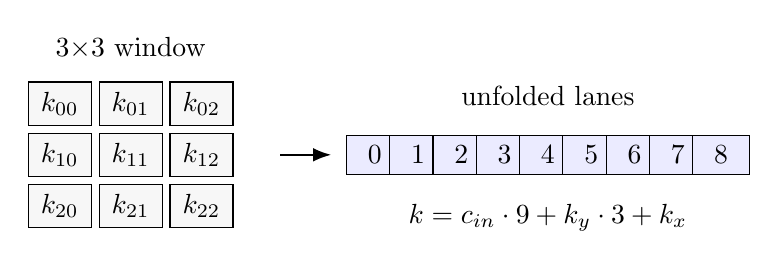
\begin{tikzpicture}[
    >=Latex,
    cell/.style={draw, minimum width=0.8cm, minimum height=0.55cm, fill=black!3},
    lane/.style={draw, minimum width=0.72cm, minimum height=0.5cm, fill=blue!8},
    arr/.style={->, thick}
]
    \foreach \y in {0,1,2} {
        \foreach \x in {0,1,2} {
            \node[cell] (c\y\x) at (\x*0.9,-\y*0.65) {$k_{\y\x}$};
        }
    }
    \node[above] at (0.9,0.45) {3$\times$3 window};
    \foreach \i in {0,...,8} {
        \node[lane] (l\i) at (4.0+\i*0.55, -0.65) {$\i$};
    }
    \draw[arr] (2.8,-0.65) -- (3.45,-0.65);
    \node[above] at (6.2,-0.15) {unfolded lanes};
    \node[below] at (6.2,-1.15) {$k=c_{in}\cdot9+k_y\cdot3+k_x$};
\end{tikzpicture}
\caption{3$\times$3 窗口到 unfolded lane 的映射}
\label{fig:window_lane_report}
\end{figure}

\section{窗口就绪与背压}

输入前端包含两个重要控制条件：

\begin{itemize}
    \item \textbf{window ready}：当前窗口需要的输入行已经在 line buffer 中就绪，或者该行属于 padding 区域。
    \item \textbf{IFM FIFO not full}：下游 IFM FIFO 仍有空间接收当前窗口展开结果。
\end{itemize}

只有当两个条件同时满足时，窗口流控制器才推进 $ox$，并向 IFM FIFO 写入一拍 lane 数据。否则输出坐标暂停，等待行填充或下游缓冲释放。这保证了输入窗口生成不会覆盖尚未消费的数据，也不会在输入行未准备好时生成错误窗口。

\chapter{三级分块调度与 Layer Scheduler}

\section{PPT 展示重点}

\begin{itemize}
    \item Layer scheduler 是把数学分块变成硬件执行序列的核心控制器。
    \item 外层按 Cout block 迭代，内层按 K pass 迭代。
    \item 每个 K pass 包含 weight load、window feeder、systolic compute、PSUM drain。
    \item Spatial tile 由外部配置多次启动，每次只处理一段输出行。
    \item start/done/clear 构成每个 tile 的启动和完成契约。
\end{itemize}

\section{调度层级}

硬件 IP 内部一次 start 对应一个 spatial tile。每次 tile 内部，调度器执行：

\begin{equation}
\begin{aligned}
&\text{for } cout\_base = 0,\COUTTILE,2\COUTTILE,\dots\\
&\quad \text{load bias block}\\
&\quad \text{for } pass\_base\_k = 0,\KTILE,2\KTILE,\dots\\
&\quad\quad \text{load weight tile}\\
&\quad\quad \text{feed IFM windows}\\
&\quad\quad \text{run systolic compute}\\
&\quad\quad \text{drain PSUM}
\end{aligned}
\end{equation}

其中 bias 只在每个 Cout block 开始时加载一次；weight tile 每个 K pass 都需要加载，因为当前 K 范围不同；IFM window 由 feeder 根据当前 pass 和输出像素范围生成。

\section{状态机流程}

\begin{figure}[htbp]
\centering
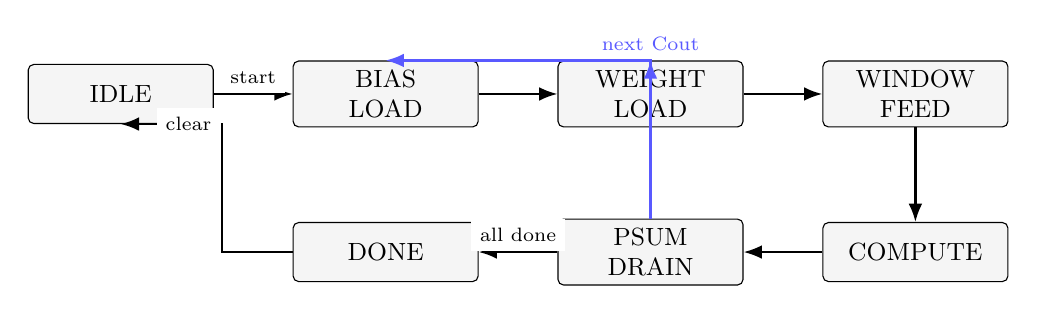
\begin{tikzpicture}[
    >=Latex,
    state/.style={draw, rounded corners=2pt, minimum width=2.35cm, minimum height=0.75cm, align=center, fill=black!4, font=\small},
    arr/.style={->, thick},
    loop/.style={->, thick, blue!65},
    cond/.style={font=\scriptsize, fill=white}
]
    \node[state] (idle) {IDLE};
    \node[state, right=of idle] (bias) {BIAS\\LOAD};
    \node[state, right=of bias] (wgt) {WEIGHT\\LOAD};
    \node[state, right=of wgt] (feed) {WINDOW\\FEED};
    \node[state, below=1.2cm of feed] (comp) {COMPUTE};
    \node[state, left=of comp] (drain) {PSUM\\DRAIN};
    \node[state, left=of drain] (done) {DONE};

    \draw[arr] (idle) -- node[cond, above]{start} (bias);
    \draw[arr] (bias) -- (wgt);
    \draw[arr] (wgt) -- (feed);
    \draw[arr] (feed) -- (comp);
    \draw[arr] (comp) -- (drain);
    \draw[loop] (drain.north) |- node[cond, above]{next K} (wgt.north);
    \draw[loop] (drain.north) |- node[cond, above]{next Cout} (bias.north);
    \draw[arr] (drain) -- node[cond, above]{all done} (done);
    \draw[arr] (done.west) -- ++(-0.9,0) |- node[cond, left]{clear} (idle.south);
\end{tikzpicture}
\caption{Layer scheduler 抽象状态机}
\label{fig:scheduler_report}
\end{figure}

\section{K pass 语义}

K pass 是多轮累加的核心。设第 $t$ 个 pass 的 K 范围为：

\begin{equation}
k \in [t\KTILE,\ (t+1)\KTILE).
\end{equation}

则每个 pass 完成：

\begin{equation}
PSUM_t[p,c] =
PSUM_{t-1}[p,c] +
\sum_{r=0}^{\KTILE-1}
IFM[p,t\KTILE+r]\cdot W[t\KTILE+r,c].
\end{equation}

其中：

\begin{equation}
PSUM_{-1}[p,c] = Bias[c].
\end{equation}

最终输出为：

\begin{equation}
OFM_{psum}[p,c] = PSUM_{N_K-1}[p,c].
\end{equation}

硬件上，$PSUM_{t-1}$ 由 feedback buffer 提供；当 $t=0$ 时由 bias buffer 提供。

\section{Spatial tile 语义}

Spatial tile 用于限制一次 start 覆盖的输出像素数。配置项包括：

\begin{itemize}
    \item \signal{tile\_oy\_base}：当前 tile 的全局输出起始行。
    \item \signal{tile\_ofm\_h}：当前 tile 覆盖的输出行数。
    \item \signal{num\_pixels}：当前 tile 的输出像素数。
    \item \signal{tile\_pixel\_base}：当前 tile 在全局 HWC OFM 中的像素基址。
\end{itemize}

这些参数使硬件无需知道完整网络调度，只需完成当前 tile。多个 tile 的启动顺序可由外部控制，最终通过 HWC 地址自然拼接为完整 OFM。

\chapter{PSUM 反馈与后处理流水线}

\section{PPT 展示重点}

\begin{itemize}
    \item PSUM 反馈路径保证多 K pass 的累加语义。
    \item 非最终 pass 的 PSUM 留在片上反馈缓冲，最终 pass 的 PSUM 进入后处理。
    \item Requant 将 INT32 PSUM 转为 INT8 OFM。
    \item Activation 支持 bypass、ReLU、Leaky LUT。
    \item Writeback 按 HWC 布局生成 byte 地址。
\end{itemize}

\section{PSUM packet 格式}

阵列底部每个输出像素产生一个 $COUT_{\mathrm{TILE}}$ 宽的 PSUM packet：

\begin{equation}
\begin{aligned}
Packet(p,cout\_base)=
\{&PSUM[p,cout\_base+0],\dots,\\
  &PSUM[p,cout\_base+\COUTTILE-1]\}.
\end{aligned}
\end{equation}

当最后一个 Cout block 不满 $\COUTTILE$ 时，通过 channel valid mask 标记有效 lane，写回阶段只输出有效通道。

\section{反馈路径}

反馈路径的抽象流程如下：

\begin{figure}[htbp]
\centering
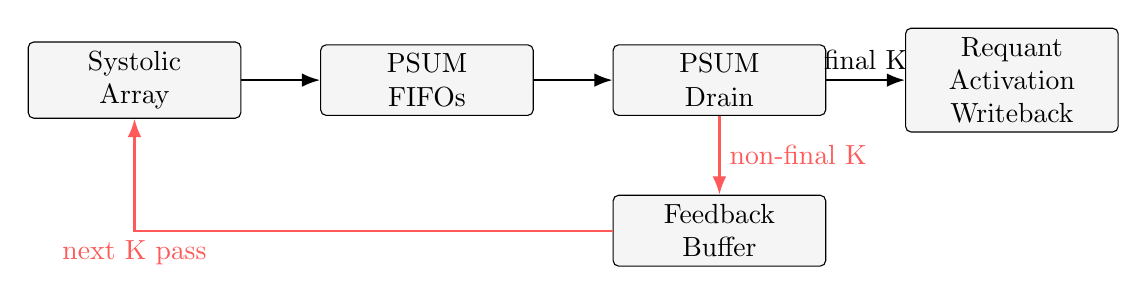
\begin{tikzpicture}[
    >=Latex,
    block/.style={draw, rounded corners=2pt, align=center, minimum width=2.7cm, minimum height=0.8cm, fill=black!4},
    arr/.style={->, thick},
    redarr/.style={->, thick, red!65}
]
    \node[block] (array) {Systolic\\Array};
    \node[block, right=of array] (fifo) {PSUM\\FIFOs};
    \node[block, right=of fifo] (drain) {PSUM\\Drain};
    \node[block, below=1.0cm of drain] (fb) {Feedback\\Buffer};
    \node[block, right=of drain] (post) {Requant\\Activation\\Writeback};

    \draw[arr] (array) -- (fifo);
    \draw[arr] (fifo) -- (drain);
    \draw[redarr] (drain) -- node[right]{non-final K} (fb);
    \draw[redarr] (fb.west) -| node[below]{next K pass} (array.south);
    \draw[arr] (drain) -- node[above]{final K} (post);
\end{tikzpicture}
\caption{PSUM 在非最终 K pass 与最终 K pass 中的去向}
\label{fig:psum_feedback_report}
\end{figure}

从汇报角度，应特别说明：反馈路径是使小阵列覆盖长 K 维度的关键。如果没有这条路径，那么每个 K tile 的结果必须写回片外再读回，带宽和延迟都会显著增加。

\section{重量化公式}

阵列输出 PSUM 为 32 bit 有符号整数。重量化模块按输出通道配置乘数、移位和零点：

\begin{equation}
y_q =
\mathrm{clip}_{[-128,127]}
\left(
\left(
psum \times mult + round
\right) \gg shift
 + zp
\right).
\label{eq:requant_report}
\end{equation}

其中 $mult$ 为 16 bit 定点乘数，$shift$ 为右移量，$zp$ 为输出零点。硬件上对 $\COUTTILE$ 个 lane 并行实例化重量化路径，使一个 final PSUM packet 可以流水化转换为一个 OFM packet。

\section{激活函数}

激活模块支持三种模式：

\begin{table}[htbp]
\centering
\caption{激活模式}
\label{tab:activation_modes}
\begin{tabular}{lll}
\toprule
\textbf{mode} & \textbf{名称} & \textbf{硬件实现} \\
\midrule
0 & bypass & 直接输出重量化结果 \\
1 & ReLU & 若 signed INT8 小于 0，则输出 0 \\
2 & Leaky LUT & 使用 256-entry 查找表完成非线性映射 \\
\bottomrule
\end{tabular}
\end{table}

这部分在 PPT 中不需要展开为过多数学推导，重点说明它已经被集成在 IP 后端，最终输出不是裸 PSUM，而是经过量化和激活后的 INT8 OFM。

\section{HWC 写回地址}

OFM 写回采用 HWC 布局。对 tile 内像素 $local\_pixel$ 和通道 lane，有：

\begin{equation}
wr\_addr =
(tile\_pixel\_base + local\_pixel)\cdot cout\_total
+ (cout\_base + lane).
\label{eq:writeback_report}
\end{equation}

这个公式同时解决 spatial tile 和 Cout block 的拼接问题。前者改变全局像素基址，后者改变输出通道基址，二者最终在同一个 HWC 地址公式中合成。

\chapter{AXI 边界与硬件 IP 封装}

\section{PPT 展示重点}

\begin{itemize}
    \item AXI-Lite 负责配置寄存器和状态查询。
    \item AXI-Stream 负责 bias、weight、IFM line 和 OFM 输出四条数据路径。
    \item 数据流接口先按调试友好格式实现，再保留后续高带宽打包优化空间。
    \item 接口层是硬件 IP 边界，不在本报告中展开完整软件系统。
\end{itemize}

\section{AXI-Lite 配置寄存器}

当前 layer 配置寄存器包括尺寸、卷积参数、分块参数和状态控制。核心寄存器如下：

\begin{table}[htbp]
\centering
\caption{核心配置寄存器}
\label{tab:reg_report}
\begin{tabular}{cll}
\toprule
\textbf{地址} & \textbf{名称} & \textbf{含义} \\
\midrule
0x00 & CTRL/STATUS & start、clear done、busy、done sticky \\
0x01 & FM\_SIZE & 输入特征图高宽 \\
0x02 & OFM\_SIZE & 输出特征图高宽 \\
0x03 & CONV & stride、pad \\
0x04 & K\_TOTAL & 展开输入维度总量 \\
0x05 & COUT\_TOTAL & 输出通道总量 \\
0x06 & NUM\_PIXELS & 当前 spatial tile 像素数 \\
0x07 & ACT\_CFG & 激活模式 \\
0x08 & TILE\_ROWS & tile 起始输出行和 tile 高度 \\
0x09 & PIXEL\_BASE & tile 全局像素基址 \\
\bottomrule
\end{tabular}
\end{table}

AXI-Lite bridge 的实现重点包括 AW/W 分离握手、WSTRB 字节合并、读写响应以及 start pulse 的单周期化。这些细节保证配置接口符合 AXI-Lite 基本时序要求。

\section{AXI-Stream 打包协议}

四条数据流的 64 bit 打包方式如下：

\begin{table}[htbp]
\centering
\caption{AXI-Stream 数据流打包方式}
\label{tab:axis_pack_report}
\begin{tabular}{lll}
\toprule
\textbf{流} & \textbf{TDATA 含义} & \textbf{TLAST 语义} \\
\midrule
Bias & 2 个 32 bit bias & 一个 Cout block 结束 \\
Weight & 8 个 INT8 weight & 一个 weight tile 结束 \\
IFM line & bank 字节，低 40 bit 有效 & 一行 IFM 结束 \\
OFM debug & byte address + byte data & 一个 spatial tile 输出结束 \\
\bottomrule
\end{tabular}
\end{table}

其中 OFM debug stream 当前采用调试友好格式：每个 beat 只携带一个 OFM byte 及其地址。这种格式带宽利用率不高，但验证非常直接。后续若追求端到端性能，应将 OFM 输出优化为连续 HWC byte 的 64 bit 或 128 bit burst stream。

\section{OFM 背压链}

OFM 输出侧存在下游 \signal{tready} 拉低的可能。为避免数据丢失，后处理链路中加入了 packet FIFO 和 byte FIFO，将背压从 AXI-Stream 边界向上游传播：

\begin{equation}
\begin{aligned}
\signal{ofm\_tready}
&\rightarrow \module{ofm\_byte\_stream\_fifo}
\rightarrow \module{ofm\_writeback}
\rightarrow \module{ofm\_packet\_fifo}\\
&\rightarrow \module{ofm\_activation}
\rightarrow \module{psum\_packet\_fifo}
\rightarrow \module{psum\_drain\_writer}.
\end{aligned}
\end{equation}

当前验证目标是支持短 burst 型背压，即 DMA 短时间停收时不丢数据。若未来系统中输出 DMA 可能长时间不可用，则需要进一步增加 FIFO 深度或在调度层限制后端积压。

\chapter{验证方法与资源评估}

\section{PPT 展示重点}

\begin{itemize}
    \item 验证采用 Icarus Verilog 模块级快速回归和 Vivado XSIM 系统级长回归。
    \item 覆盖 PE、窗口、调度、PSUM 反馈、量化激活、AXI 边界和背压场景。
    \item 资源评估比较 32$\times$32、32$\times$16、16$\times$16、18$\times$16。
    \item 18$\times$16 是 XCK26 上资源与性能折中的最终实现点。
\end{itemize}

\section{验证层次}

验证工作按三层组织：

\begin{enumerate}
    \item \textbf{模块级验证}：针对 PE、FIFO、line buffer、window feeder、requant、activation、writeback、AXI wrapper 等独立模块建立小 testbench。
    \item \textbf{核心链路验证}：覆盖 systolic top、feeder、scheduler、PSUM drain/feedback、multi-pass 和 Cout block。
    \item \textbf{端到端验证}：通过 AXI-Lite/AXI-Stream 版本 PS driver，覆盖多 spatial tile、多 K pass、多 Cout block 和 OFM backpressure。
\end{enumerate}

所有系统级测试均与 golden convolution 结果比较，重点检查全局 HWC OFM memory 是否完全一致。

\section{典型覆盖场景}

\begin{table}[htbp]
\centering
\caption{关键验证场景}
\label{tab:verify_report}
\begin{tabular}{lp{0.62\textwidth}}
\toprule
\textbf{场景} & \textbf{覆盖内容} \\
\midrule
window feeder pad/stride & padding 输出 0、stride 坐标映射、窗口 ready 判断 \\
multi-pass systolic & K pass 之间 PSUM 反馈与重新注入 \\
Cout block & 输出通道超过 $\COUTTILE$ 时的权重重载和地址偏移 \\
spatial multi-tile & 多个输出行 tile 拼接到全局 HWC OFM \\
AXI-Lite PS driver & 寄存器配置、start/done/clear 调度契约 \\
AXI-Stream PS driver & bias、weight、IFM、OFM 四路 AXI 边界 \\
backpressure & OFM downstream ready 短暂停顿下的数据完整性 \\
\bottomrule
\end{tabular}
\end{table}

\section{资源配置对比}

\begin{table}[htbp]
\centering
\caption{XCK26 四种阵列配置资源评估}
\label{tab:resource_report}
\begin{tabular}{lcccccc}
\toprule
\textbf{配置} & \textbf{K tile} & \textbf{Cout tile} & \textbf{LUT} & \textbf{DSP} & \textbf{BRAM} & \textbf{时序} \\
\midrule
32$\times$32 & 32 & 64 & 196.83\% & 92.55\% & 61.81\% & WNS +1.809 ns \\
32$\times$16 & 32 & 32 & 105.77\% & 46.39\% & 30.90\% & WNS +1.873 ns \\
16$\times$16 & 16 & 32 & 60.62\% & 25.88\% & 30.90\% & WNS +2.144 ns \\
18$\times$16 & 18 & 32 & 62.39\% & 28.45\% & 30.90\% & routed WNS +0.262 ns \\
\bottomrule
\end{tabular}
\end{table}

从资源结果看，32$\times$32 满规模阵列理论吞吐最高，但无法装入 XCK26；32$\times$16 保留了 32 行 K tile，但 LUT 仍略超；16$\times$16 最稳妥，但 K pass 数增加；18$\times$16 在 LUT/DSP 增量较小的情况下提高了 K tile 覆盖能力，并完成布局布线，因此作为当前最终实现点。

\section{资源瓶颈讨论}

LUT 是当前最主要瓶颈。主要来源包括：

\begin{itemize}
    \item 阵列内部 valid skew 和 IFM/PSUM 延迟链。
    \item 多 lane window extract 的组合选择逻辑。
    \item 多路 packet FIFO、activation LUT 和 OFM debug writer。
    \item 双 INT8 DSP 封装周围的符号校正和旁路逻辑。
\end{itemize}

后续优化方向包括：用集中式计数控制替代大量分布式延迟链；将 Leaky LUT、debug writer 等模块参数化裁剪；优化 OFM 输出为连续 burst；重新探索 ROWS/COLS 的非整十六配置。

\chapter{PPT 制作建议与页面拆分}

\section{推荐页面结构}

根据以上技术报告内容，正式 PPT 可拆成 14 到 18 页：

\begin{enumerate}
    \item 标题页：课题、平台、核心关键词。
    \item 问题背景：边缘 CNN 推理瓶颈。
    \item 设计目标：硬件 IP 的功能边界和目标器件。
    \item 卷积到 GEMM：核心公式和展开维度。
    \item 三级分块：K/Cout/Spatial 分块图。
    \item 总体架构：完整硬件数据流框图。
    \item PE 结构：双权重、IFM/PSUM 传播。
    \item 阵列数据流：weight-stationary 的二维方向图。
    \item 输入前端：line buffer + window extract。
    \item 调度状态机：layer scheduler 流程。
    \item PSUM 反馈：多 K pass 累加语义。
    \item 后处理：requant、activation、HWC writeback。
    \item AXI 边界：配置寄存器和四路 stream。
    \item 验证方法：模块级到端到端。
    \item 资源结果：四种配置对比。
    \item 总结：贡献、限制和后续优化。
\end{enumerate}

\section{讲述节奏建议}

如果汇报时间为 10 分钟，建议弱化接口细节和验证表格，只保留架构、阵列、分块和资源结论。若汇报时间为 20 分钟，可以完整讲清公式、数据流、状态机和 PSUM 反馈。若用于论文预答辩，则建议保留第 2 章至第 8 章的完整技术链路，并把第 9 章作为 PPT 制作索引。

\section{总结陈述}

本硬件 IP 的核心价值在于将 CNN 卷积层拆解为一套可在 FPGA 上稳定执行的流式数据通路。它使用 weight-stationary 脉动阵列承担主要乘加计算，用行缓存和窗口提取避免显式 im2col 存储，用三级分块解决阵列规模有限的问题，用片上 PSUM 反馈保持多 pass 累加语义，并通过后处理和 AXI 边界形成可验证、可综合、可部署的硬件 IP 形态。

\end{document}
